\documentclass[a4paper,11pt]{exam}
\printanswers % pour imprimer les réponses (corrigé)
% \noprintanswers % Pour ne pas imprimer les réponses (énoncé)
%\addpoints % Pour compter les points
 \noaddpoints % pour ne pas compter les points
\qformat{\textbf{\thequestion ) } }
%\qformat{\textbf{Question\thequestion}\quad(\thepoints)\hfill} % Pour définir le style des questions (facultatif)
\usepackage{color} % définit une nouvelle couleur
\shadedsolutions % définit le style des réponses
% \framedsolutions % définit le style des réponses
\definecolor{SolutionColor}{rgb}{0.8,0.9,1} % bleu ciel
\renewcommand{\solutiontitle}{\noindent\textbf{Solution:}\par\noindent} % Définit le titre des solutions


%\usepackage{../../pas-math}
%\usepackage{../../moncours}


%\usepackage{pas-cours}
%-------------------------------------------------------------------------------
%          -Packages nécessaires pour écrire en Français et en UTF8-
%-------------------------------------------------------------------------------
\usepackage[utf8]{inputenc}
\usepackage[frenchb]{babel}
\usepackage[T1]{fontenc}
\usepackage{lmodern}
\usepackage{textcomp}



%-------------------------------------------------------------------------------

%-------------------------------------------------------------------------------
%                          -Outils de mise en forme-
%-------------------------------------------------------------------------------
\usepackage{hyperref}
\hypersetup{pdfstartview=XYZ}
%\usepackage{enumerate}
\usepackage{graphicx}
\usepackage{multicol}
\usepackage{tabularx}
\usepackage{multirow}


\usepackage{anysize} %%pour pouvoir mettre les marges qu'on veut
%\marginsize{2.5cm}{2.5cm}{2.5cm}{2.5cm}

\usepackage{indentfirst} %%pour que les premier paragraphes soient aussi indentés
\usepackage{verbatim}
\usepackage{enumitem}
\usepackage[usenames,dvipsnames,svgnames,table]{xcolor}

\usepackage{variations}

%-------------------------------------------------------------------------------


%-------------------------------------------------------------------------------
%                  -Nécessaires pour écrire des mathématiques-
%-------------------------------------------------------------------------------
\usepackage{amsfonts}
\usepackage{amssymb}
\usepackage{amsmath}
\usepackage{amsthm}
\usepackage{tikz}
\usepackage{xlop}
%-------------------------------------------------------------------------------



%-------------------------------------------------------------------------------


%-------------------------------------------------------------------------------
%                    - Mise en forme avancée
%-------------------------------------------------------------------------------

\usepackage{ifthen}
\usepackage{ifmtarg}


\newcommand{\ifTrue}[2]{\ifthenelse{\equal{#1}{true}}{#2}{$\qquad \qquad$}}

%-------------------------------------------------------------------------------

%-------------------------------------------------------------------------------
%                     -Mise en forme d'exercices-
%-------------------------------------------------------------------------------
%\newtheoremstyle{exostyle}
%{\topsep}% espace avant
%{\topsep}% espace apres
%{}% Police utilisee par le style de thm
%{}% Indentation (vide = aucune, \parindent = indentation paragraphe)
%{\bfseries}% Police du titre de thm
%{.}% Signe de ponctuation apres le titre du thm
%{ }% Espace apres le titre du thm (\newline = linebreak)
%{\thmname{#1}\thmnumber{ #2}\thmnote{. \normalfont{\textit{#3}}}}% composants du titre du thm : \thmname = nom du thm, \thmnumber = numéro du thm, \thmnote = sous-titre du thm

%\theoremstyle{exostyle}
%\newtheorem{exercice}{Exercice}
%
%\newenvironment{questions}{
%\begin{enumerate}[\hspace{12pt}\bfseries\itshape a.]}{\end{enumerate}
%} %mettre un 1 à la place du a si on veut des numéros au lieu de lettres pour les questions 
%-------------------------------------------------------------------------------

%-------------------------------------------------------------------------------
%                    - Mise en forme de tableaux -
%-------------------------------------------------------------------------------

\renewcommand{\arraystretch}{1.7}

\setlength{\tabcolsep}{1.2cm}

%-------------------------------------------------------------------------------



%-------------------------------------------------------------------------------
%                    - Racourcis d'écriture -
%-------------------------------------------------------------------------------

% Angles orientés (couples de vecteurs)
\newcommand{\aopp}[2]{(\vec{#1}, \vec{#2})} %Les deuc vecteurs sont positifs
\newcommand{\aopn}[2]{(\vec{#1}, -\vec{#2})} %Le second vecteur est négatif
\newcommand{\aonp}[2]{(-\vec{#1}, \vec{#2})} %Le premier vecteur est négatif
\newcommand{\aonn}[2]{(-\vec{#1}, -\vec{#2})} %Les deux vecteurs sont négatifs

%Ensembles mathématiques
\newcommand{\naturels}{\mathbb{N}} %Nombres naturels
\newcommand{\relatifs}{\mathbb{Z}} %Nombres relatifs
\newcommand{\rationnels}{\mathbb{Q}} %Nombres rationnels
\newcommand{\reels}{\mathbb{R}} %Nombres réels
\newcommand{\complexes}{\mathbb{C}} %Nombres complexes


%Intégration des parenthèses aux cosinus
\newcommand{\cosP}[1]{\cos\left(#1\right)}
\newcommand{\sinP}[1]{\sin\left(#1\right)}


%Probas stats
\newcommand{\stat}{statistique}
\newcommand{\stats}{statistiques}
%-------------------------------------------------------------------------------

%-------------------------------------------------------------------------------
%                    - Mise en page -
%-------------------------------------------------------------------------------

\newcommand{\twoCol}[1]{\begin{multicols}{2}#1\end{multicols}}


\setenumerate[1]{font=\bfseries,label=\textit{\alph*})}
\setenumerate[2]{font=\bfseries,label=\arabic*)}


%-------------------------------------------------------------------------------
%                    - Elements cours -
%-------------------------------------------------------------------------------





%\usepackage{fullpage}
\author{\ }
\date{27 Septembre 2016}
\title{DS num\'ero 1}


\begin{document}
	
	\maketitle
\section{Prix d'un vélo}
	
	
	L'étude suivante porte sur le prix d'un vélo dans 50 points de vente différents.
	
	\begin{center}
		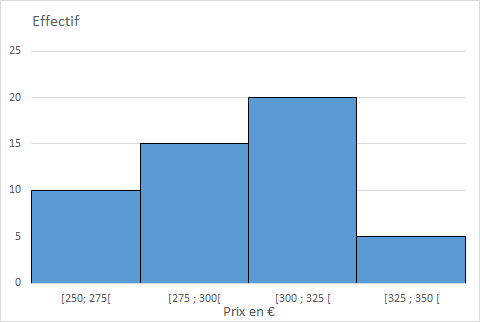
\includegraphics[scale=0.55]{./histo}
	\end{center}
		
		
				
		\begin{table}[h]
			\centering
			%\caption{}
			\label{my-label}
			\begin{tabular}{|@{\ }c@{\ }|@{\ }c@{\ }|@{\ }c@{\ }|@{\ }c@{\ }|@{\ }c@{\ }|}
				\hline
				\textbf{Prix} (en €) & [250 ; 275[ & [275 ; 300[ & [300 ; 325 [  & [325 ; 350 [\\
				\hline
				\textbf{Effectif} &  &  &  & \\
				\hline 
			\end{tabular}
		\end{table}
	
	
	%\begin{multicols}{2}
		
		

	\begin{questions} % Début de l'examen
		
		\question Donner le caractère étudié et sa nature.
		\begin{solution}
			Le caractère étudié est le prix d'un vélo ; il est quantitatif.
		\end{solution}
		
		\question Reporter les effectifs dans le tableau.
		\begin{solution}
			
				\begin{tabular}{|@{\ }c@{\ }|@{\ }c@{\ }|@{\ }c@{\ }|@{\ }c@{\ }|@{\ }c@{\ }|}
					\hline
					\textbf{Prix} (en €) & [250 ; 275[ & [275 ; 300[ & [300 ; 325 [  & [325 ; 350 [\\
					\hline
					\textbf{Effectif} & 10 & 15  & 20 &  5\\
					\hline 
				\end{tabular}
			
		\end{solution}
		
		\question Quel est l'effectif total ?
		\begin{solution}
			L'effectif total est 50.
		\end{solution}
		
		\question Combien de magasins vendent des vélos à moins de 300 euros ?
		\begin{solution}
			25 magasins vendent des vélos à moins de 300 euros.
		\end{solution}
		
		\question Calculer le nombre de magasins où des vélos sont vendus à un prix d'au moins 300 euros.
		\begin{solution}
			25 magasins vendent des vélos à au moins 300 euros.
		\end{solution}
	\end{questions}
%\end{multicols}

\newpage

\section{Diner de gala}

	\begin{multicols}{2}
		\ \\
		\ \\
		Lors d'un dîner organisé pour 120 personnes, les convives pouvaient choisir parmi plusieurs desserts. La répartition s'effectue de la manière suivante :
		
		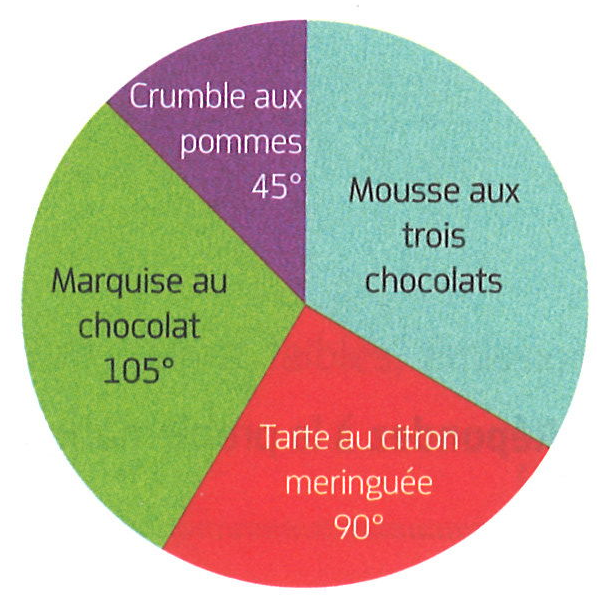
\includegraphics[scale=0.8]{./secteurs}
		
		
	\end{multicols}
	 
	\begin{questions}
		\question A l'aide du diagramme, recopier et compléter le tableau suivant :
	
		\begin{footnotesize}
			\begin{tabular}{|@{\ }c@{\ }|@{\ }c@{\ }|@{\ }c@{\ }|@{\ }c@{\ }|@{\ }c@{\ }|@{\ }c@{\ }|}
				\hline
				\textbf{Dessert} & \textbf{Crumble aux pommes} & \textbf{Mousse aux 3 chocolats} & \textbf{Tarte au citron}  & \textbf{Marquise au chocolat} & \textbf{Total}\\
				\hline
				\textbf{Effectif} &  &   &  &  & \\
				\hline
				\textbf{Angle} &  &   &  &  & 360°\\ 
				\hline
			\end{tabular}
		\end{footnotesize}
	
		
		
		\begin{solution}
			\begin{footnotesize}
				\begin{tabular}{|@{\ }c@{\ }|@{\ }c@{\ }|@{\ }c@{\ }|@{\ }c@{\ }|@{\ }c@{\ }|@{\ }c@{\ }|}
					\hline
					\textbf{Dessert} & \textbf{Crumble aux pommes} & \textbf{Mousse aux 3 chocolats} & \textbf{Tarte au citron}  & \textbf{Marquise au chocolat} & \textbf{Total}\\
					\hline
					\textbf{Effectif} & 15 & 40  & 30 & 35 & 120 \\
					\hline
					\textbf{Angle} & 45 & 120  & 90 & 105 & 360°\\ 
					\hline
				\end{tabular}
			\end{footnotesize}
		\end{solution}
	\end{questions}
	
\section{Séances de cinéma}

	On demande à 25 personnes combien de fois elles sont allées au cinéma pendant l'été. On obtient les réponses suivantes : \\
	
	$3 \bullet 2 \bullet 0 \bullet 1 \bullet 5 \bullet 4 \bullet 2 \bullet 2 \bullet 1 \bullet 3 \bullet 2 \bullet 1 \bullet 4 \bullet 4 \bullet 0 \bullet 1 \bullet 2 \bullet 1 \bullet 0 \bullet 0 \bullet 2 \bullet 5 \bullet 4 \bullet 1 \bullet 2$
	
	\begin{questions}
		\question Compléter le tableau suivant :
		
		\begin{center}
			\begin{tabular}{|@{\ }c@{\ }|@{\ }c@{\ }|@{\ }c@{\ }|@{\ }c@{\ }|@{\ }c@{\ }|@{\ }c@{\ }|@{\ }c@{\ }|}
				\hline
				\textbf{Nb de séances} & \ 0\  & \ 1\  & \ 2\  & \ 3\  & \ 4\  & \ 5\ \\
				\hline
				\textbf{Effectif} &  &   &  &  & &\\
				
				\hline
			\end{tabular}
		\end{center}
		
		\begin{solution}
			
			\begin{center}
				\begin{tabular}{|@{\ }c@{\ }|@{\ }c@{\ }|@{\ }c@{\ }|@{\ }c@{\ }|@{\ }c@{\ }|@{\ }c@{\ }|@{\ }c@{\ }|}
					\hline
					\textbf{Nb de séances} & \ 0\  & \ 1\  & \ 2\  & \ 3\  & \ 4\  & \ 5\ \\
					\hline
					\textbf{Effectif} & 4 & 6  & 7 & 2 & 4 & 2 \\
					
					\hline
				\end{tabular}
			\end{center}
			
		\end{solution}
		
		\question Donner le caractère étudié et sa nature.
		\begin{solution}
			Le caractère étudié est le nombre de séances de cinéma, il est quantitatif.
		\end{solution}
		
		\question Donner l'effectif total.
		\begin{solution}
			L'effectif total est 25 personnes.
		\end{solution}
		
		\question Construire le diagramme en bâtons correspondant (prendre 1 cm ou 1 carreau pour 1 séance).
		\begin{solution}
			\begin{center}
				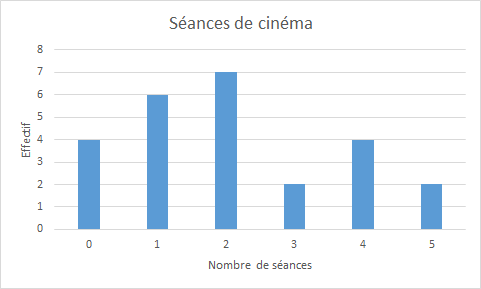
\includegraphics[scale=0.6]{./cine}
			\end{center} 
		\end{solution}
	\end{questions}
\end{document}